% Template for ICASSP-2020 paper; to be used with:
%          spconf.sty  - ICASSP/ICIP LaTeX style file, and
%          IEEEbib.bst - IEEE bibliography style file.
% --------------------------------------------------------------------------
\documentclass{article}
\usepackage{spconf,amsmath,graphicx}
\usepackage{enumerate}

% Example definitions.
% --------------------
\def\x{{\mathbf x}}
\def\L{{\cal L}}

% Title.
% ------
\title{AUTHOR GUIDELINES FOR ICASSP 2020 PROCEEDINGS MANUSCRIPTS}
%
% Single address.
% ---------------
\name{Makoto Takamatsu\thanks{https://polyp.grand-challenge.org/Databases/}}
\address{Tokyo Denki University}
%
% For example:
% ------------
%\address{School\\
%	Department\\
%	Address}
%
% Two addresses (uncomment and modify for two-address case).
% ----------------------------------------------------------
%\twoauthors
%  {A. Author-one, B. Author-two\sthanks{Thanks to XYZ agency for funding.}}
%	{School A-B\\
%	Department A-B\\
%	Address A-B}
%  {C. Author-three, D. Author-four\sthanks{The fourth author performed the work
%	while at ...}}
%	{School C-D\\
%	Department C-D\\
%	Address C-D}
%
\begin{document}
%\ninept
%
\maketitle
%
\begin{abstract}
The abstract should appear at the top of the left-hand column of text, about
0.5 inch (12 mm) below the title area and no more than 3.125 inches (80 mm) in
length.  Leave a 0.5 inch (12 mm) space between the end of the abstract and the
beginning of the main text.  The abstract should contain about 100 to 150
words, and should be identical to the abstract text submitted electronically
along with the paper cover sheet.  All manuscripts must be in English, printed
in black ink.
\end{abstract}
%
\begin{keywords}
Multi frequency extraction, semantic segmentation.
\end{keywords}
%
\section{Introduction}
\label{sec:intro}
大腸がん(CRC)は,世界中でがんによる死亡の3番目の原因である[1].CRCは,最初は良性の腺腫性ポリープ(腺腫)から発生するが,時間が経つにつれて,それらのいくつかは悪性になる.CRCの生存率は,検出された段階に依存し,I期の95$\%$の高い割合から,治療をせずに放置をしたIVおよびV期には35$\%$より低い割合に低下し致命的になる[].したがって,早期に病変やポリープを検出することがCRCの予防には不可欠である[].現在,CRC関連の死亡率を減らすための標準的なアプローチは,ポリープを探すために定期的なスクリーニングを実施することであり,大腸内視鏡検査が最適なスクリーニングツールであり,臨床医はポリープを探すために腸壁を視覚的に検査する.しかしながら,内視鏡医が限られた時間内で大量の画像を読影しなければならず非常に負担が大きく,内視鏡医の誤検出率は約25$\%$[]と誤検出が起こりやすい.近年になり,ポリープのセグメンテーションは,慎重に検査するべき潜在的な病変で覆われている領域を定義するため,臨床医が除去する可能性を高めることやポリープ検出のような弱い探索はポリープの見落としにつながる可能性があるため,内腔のセグメンテーションは探索された結腸壁の程度に関連する品質指標を確立するために使用できることから,内腔内のポリープにセグメンテーションをする研究が行われている.
\begin{figure}[t]
\begin{center}
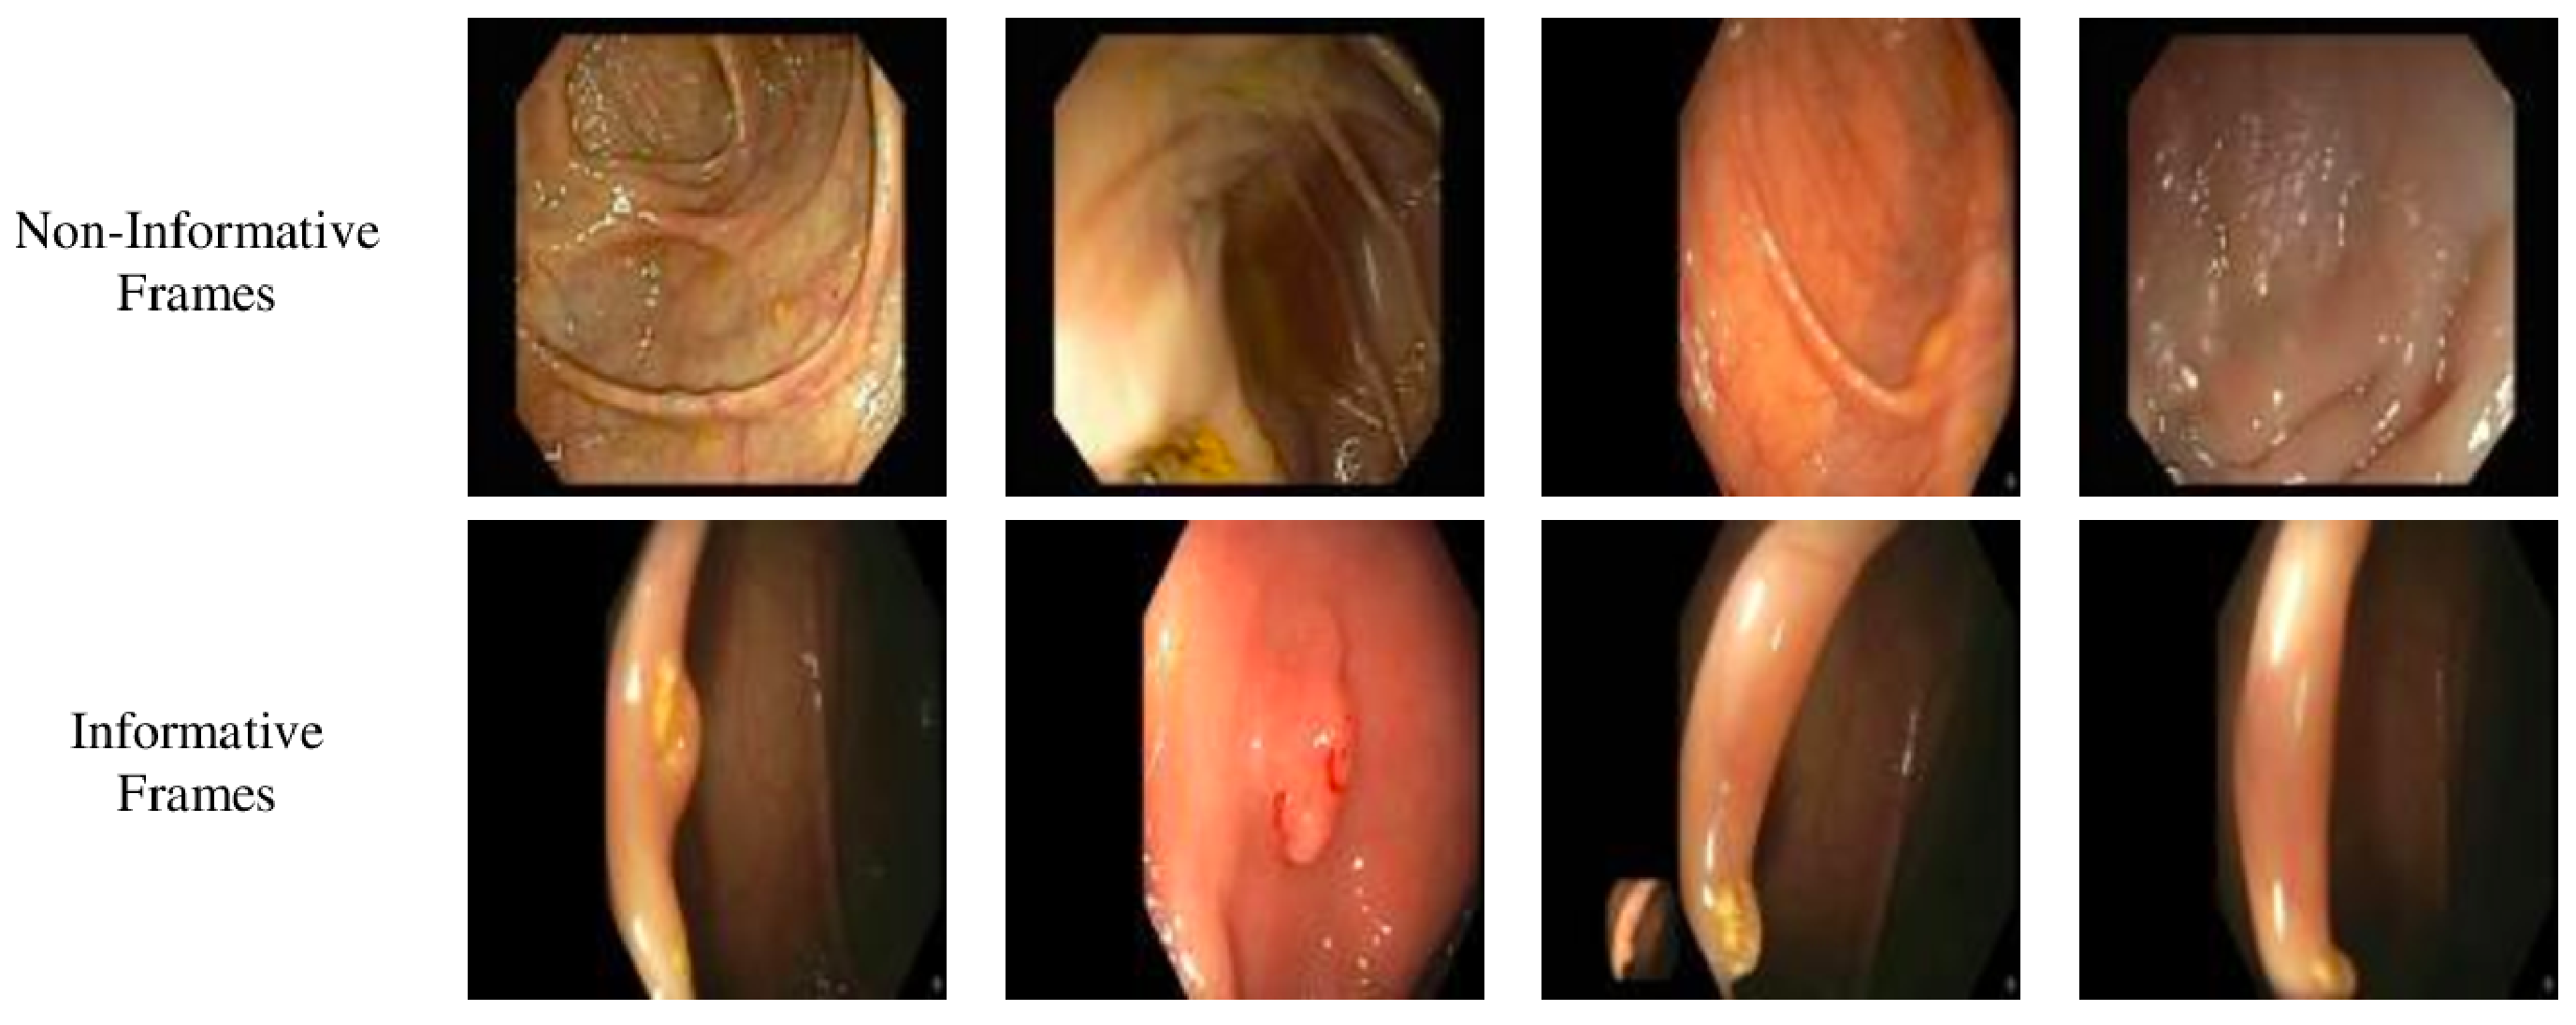
\includegraphics[width=80mm]{fig0.eps}
\caption{}
\end{center}
\end{figure}
大腸内視鏡ビデオは,キャプチャ中,腸壁が常に動き揺れているため,観察を妨げる強いボケのあるビデオをキャプチャすることがよくあり,長時間,病変に焦点を合わせ続けることが困難である.そのため,内視鏡画像には多くの弱いエッジ,テクスチャのない領域,ぼやけた領域をもつ画像が存在し,診断のパフォーマンスを大幅に妨げる.今までは,エッジ情報が豊富なシャープ画像でしかポリープの形状をセグメンテーションすることしかできなかった[],しかしながら,臨床医が実際に使用する際にはノイズにロバストなセグメンテーションができることが重要である.この作業では,激しいモーションによって引き起こされた弱いエッジ領域やぼやけた領域からも内腔内の輪郭を正確に検出し,セグメンテーションをするはじめての研究である.

セマンティックセグメンテーションでは効果的に解決するために,低レベルな特徴マップを高レベルの特徴マップと組み合わせて正確なローカライズを可能にする設計が重要である[23,24].したがって,U-netライクなネットワークで,多くのセグメンテーションタスクが取り組まれてきた.この作業では,ノイズが多い内腔内の画像からポリープの形状を正確にセグメンテーションする効果的な方法を提案する.\(1)\)画像中の複数の空間周波数特性に注目し,vanilla convolutionをOctave Convolution(OctConv)に置き換え,Residual UNetに組み込むことで,階層的特徴をデコードする.\(2)\)U-netライクなネットワークで一般的に使われているクロスエントロピー損失関数ではなく,Focal lossに変更することで,不均衡なセマンティッククラスを解消し,セグメンテーションの精度を向上させる.For example, 内視鏡のラベルでは,ポリープのピクセルは,non-polypのピクセルよりも圧倒的に小さくクラス間の不均衡が生じている.

本論文の貢献は2つである.
\begin{enumerate}[(1)]
\item 空間周波数に着目したConvolution layerを使用したモデルのほうがノイズにロバストなセグメンテーションができる事を示した.
\item 既存の手法では,非有益な画像として捨てられていたブラーフレームからもポリープの輪郭を正確に検出できる.
\end{enumerate}

The remaining sections are organixzed as following: Section2は,提案手法やセグメンテーションするためのネットワークモデル,損失関数,を説明する.section3は,pre-processingや実験方法と実験結果を示す.section4は,結論である.作成したコードは筆者のアカウントから確認できる.\texttt{https://github.com/mtakamat}.

\section{Proposed Method}
In this section,we introduce the architecture of Octave Residual UNet in full detail , a loss function design to detect more 
\label{sec:pro}
\subsection{Octave Convolution}

Octave Convolution (OctConv) layer [9]は,図のように,vanilla convolution layerを2つの解像度に分解して,特徴マップを異なる周波数マップ,低周波と高周波の特徴マップ$X = [{X^H,X^L}]$に分割する.次に,output $Y=[{Y^H,Y^L}]$of the OctConv high and low frequency feature mapは,それぞれ$Y^H=Y^{H\rightarrow H}+Y^{L\rightarrow H}$ and $Y^L=Y^{L\rightarrow L}+Y^{H\rightarrow L}$と与えられる.$Y^{H\rightarrow H},Y^{L\rightarrow L}$denote intra-frequency update, $Y^{H\rightarrow L},Y^{L\rightarrow H}$denote inter-frequency communication.
\begin{equation}
\begin{aligned} Y^{H} &=f\left(X^{H} ; W^{H \rightarrow H}\right)+ {upsample}\left(f\left(X^{L} ; W^{L \rightarrow H}\right),2)\right.\\ Y^{L} &=f\left(X^{L} ; W^{L \rightarrow L}\right)+f\left(pool\left(X^{H}, 2\right) ; W^{H \rightarrow L}\right) \end{aligned},
\end{equation}
where $f(X; W)$ denotes a convolution with parameters $W$,$ pool(X, k)$ is an average pooling operation with kernel size $k \times k$ and stride $k$. $upsample(X, k)$ is an up-sampling operation by a factor of $k$ via nearest interpolation.In practice,  the spatial dimensions of the $X^L$ feature representation are divided by a factor of 2. This further helps each OctConv layer capture more contextual information from distant locations and can potentially improve recognition performance.
\subsection{Residual Unit}
The more layers of the network, the richer the features that can be extracted. However, blindly increasing the depth of the network will lead to gradient explosions or gradient dispersion. To overcome these problem, He et al. [] proposed the residual units. Each residual unit can be illustrated as a general form  
\begin{equation}
\begin{aligned} \mathbf{y}_{l} &=h\left(\mathbf{x}_{l}\right)+\mathcal{F}\left(\mathbf{x}_{l}, \mathcal{W}_{l}\right)\\ \mathbf{x}_{l+1} &=f\left(\mathbf{y}_{l}\right) \end{aligned},
\end{equation}
where $\mathbf{x}_{l}$ and $\mathbf{x}_{l+1}$ are the input and output of the ${l}$th residual unit, $\mathcal{F}$ is the residual function, $f\left(\mathbf{y}_{l}\right)$ is the activation function, and $h$ is an identity mapping function, that is $h\left(\mathbf{x}_{l}\right)=\mathbf{x}_{l}$. He et al. []は,residual unitの様々な組み合わせの影響に関する詳細な実験を行い,図に示すfull preactivation resiaual unitを提案した.本稿では, full preactivation resiaual unitを使用してOctave Residual Unetを構築する.

\begin{figure}[t]
\begin{center}
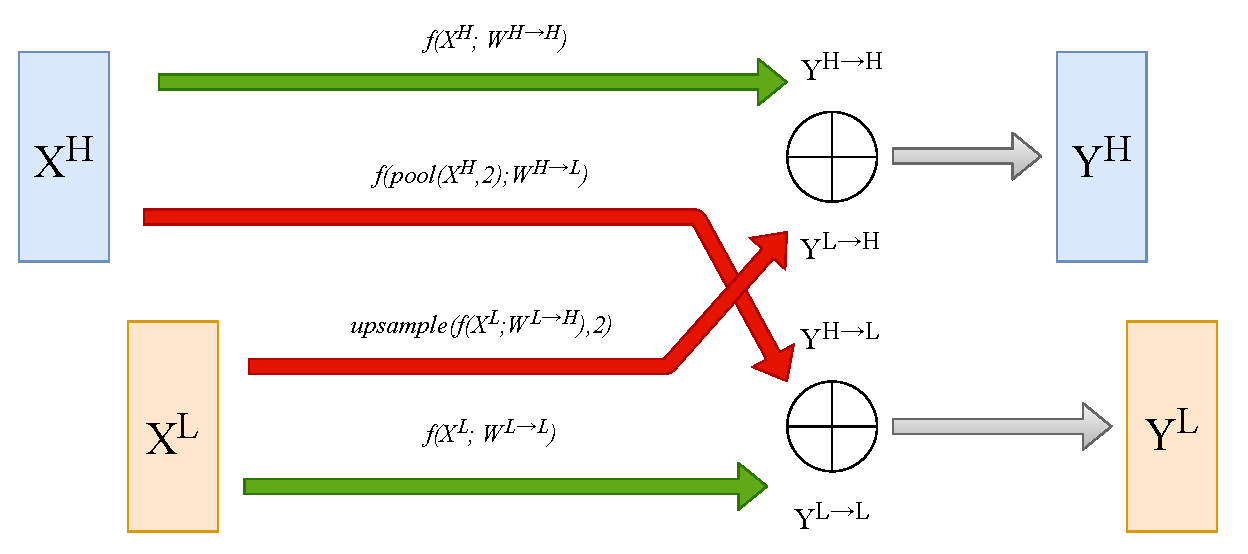
\includegraphics[width=80mm]{fig1.eps}
\caption{OctConv;Green lines indicate intra-frequency,Red lines indicate inter-frequency }
\end{center}
\end{figure}

\begin{figure}[t]
\begin{center}
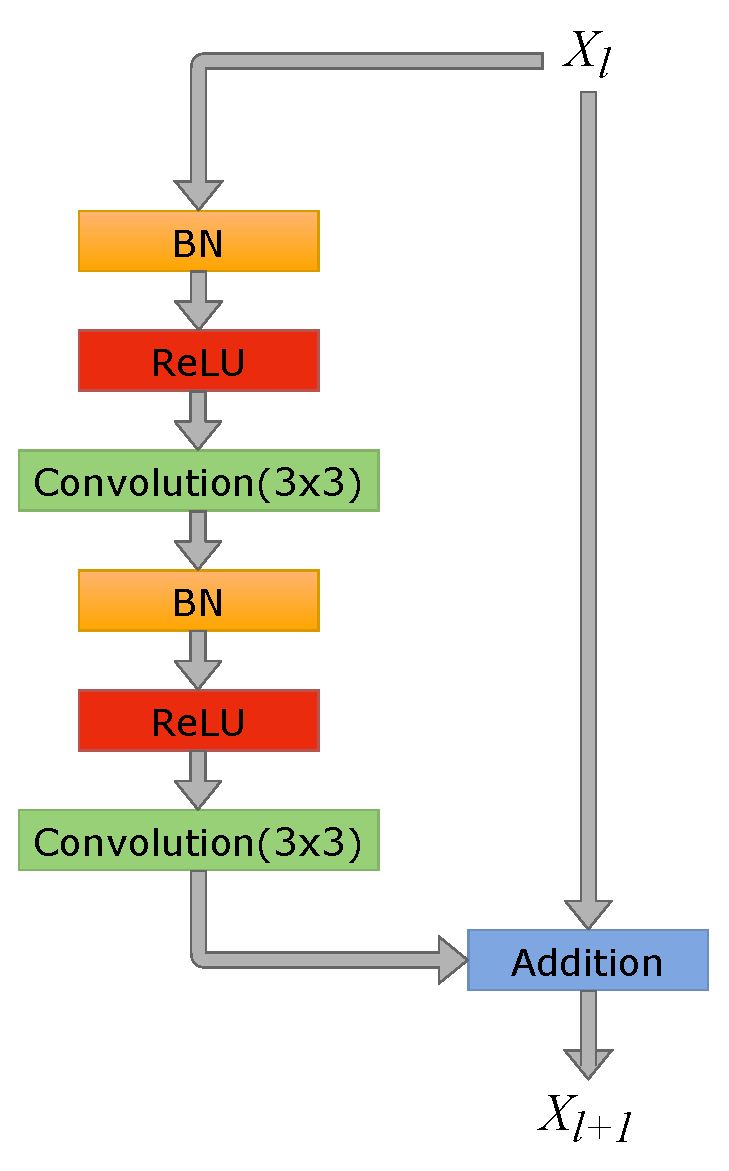
\includegraphics[width=50mm]{fig2.eps}
\caption{Residual Unit}
\end{center}
\end{figure}
\begin{figure*}[t]
\begin{center}
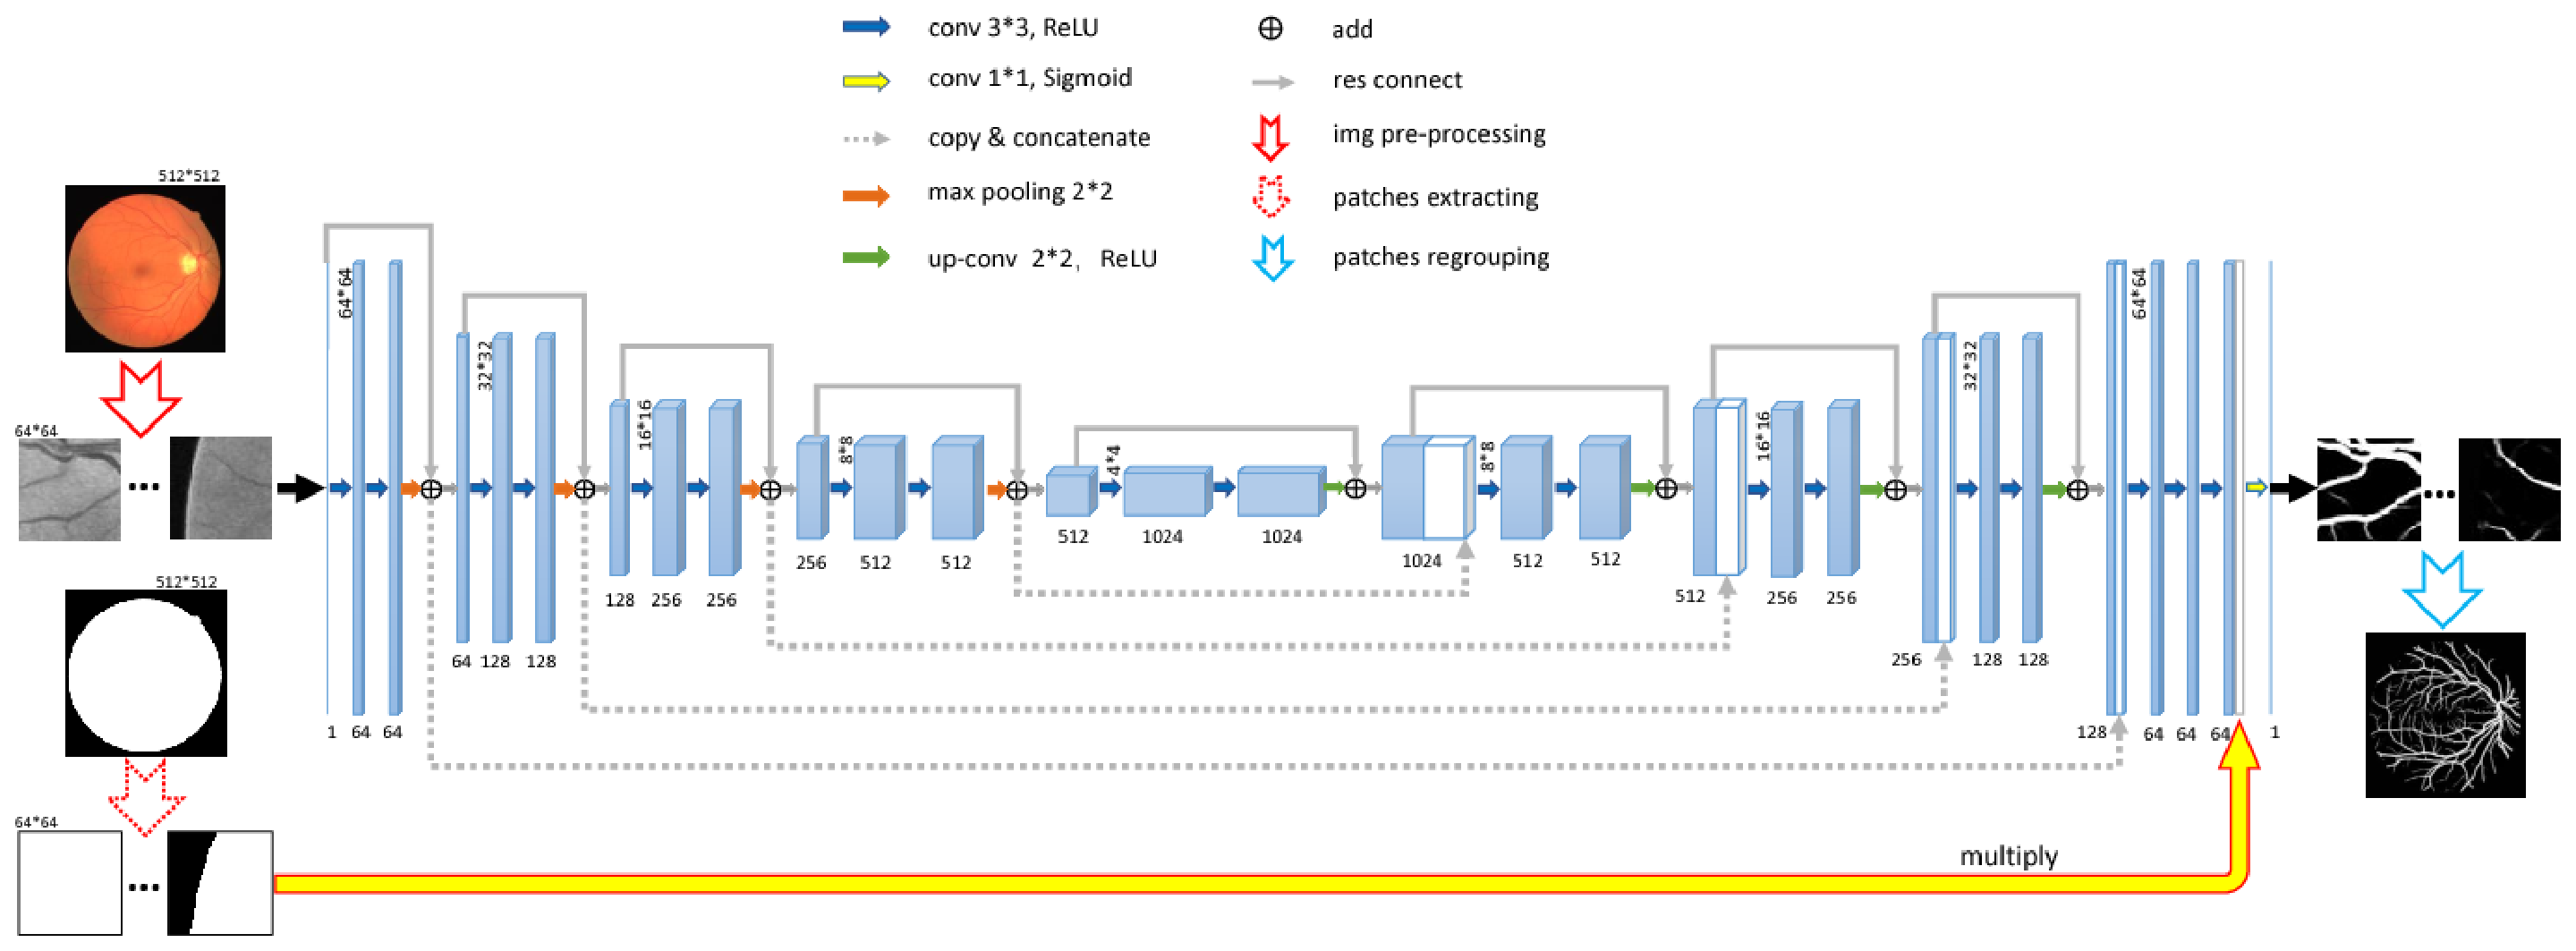
\includegraphics[width=170mm]{fig5.eps}
\caption{}
\end{center}
\end{figure*}
\subsection{Octave Residual UNet}
%OctResUNetのネットワークアーキテクチャについて説明する
In this section, Octave UNetとresidual neural networkの両方を組み合わせたencoder-decoder based neural network architecture named Octave Residul UNetを提案する [ , , ].Residual UNetの大きな利点は,residual unitおよびUnetのスキップコネクションは,情報の伝播を促進し,はるかに少ないパラメータでneural networkを設計できる上に,他のセメンティックセグメンテーションと同等の優れたパフォーマンスを達成できることである[ road,skin ].

In this paper, Octave Residual UNet is capable of extracting and decoding hierarchical multifrequency features for  segmentation polyps from blur endoscope images. Octave Residual UNet consists of 9 levels architecture,the part of Encoder, Decoder (see Fig.2).
%ここからOctave ResUnetの詳細について書く
図のように複数のエンコーダブロックを積み重ねると,滑らかに変化する構造を表す低空間周波数成分と急速に変化する詳細を表す高空間周波数成分の両方を取得できる階層型マルチ周波数特徴を抽出できる.図に示すように,特徴をエンコーディングするプロセスで,特徴マップの空間次元が徐々に減少するため,the feature maps lose spatial details and location information. Skip connections  is adopted to concatenate low level location information rich features to the inputs of decoder blocks. The stack of decoder block recovers spatial details and local information. All of the two parts are built with residual units that consist of two $3\times3$ OctConv layer and an identity mapping.

\subsubsection{Residual Down sampling block }

\subsubsection{Residual Up sampling block }
%The input image is encoded into a compact representation.The Decoder part recovers the representations to a pixel-wise categorization.The Bridge part connect the encoding and decoding paths.  All of the three parts are built with residual units that consist of two $3\times3$ OctConv layer and an identity mapping.
%できたらこれもかく.
%各ステップのパラメータと出力サイズを表に示す.

%Zhunら[]は,OctConv blockを使用したUNetを提案し,特徴マップからmultifrequency featureを抽出したエンコーダをスキップコネクションを介して表現力が低いデコーダにアクセスすることで,従来法のUNetよりも高精度に細部をセグメンテーションできることを示した.本手法は,彼らの研究をベースにしている.
\subsection{Loss Function}
Deep Learningの最適化は,損失関数によってdriveする.全体的な損失を最小にするために,Neural Networkのパラメータは,逆伝播法によって更新される.セマンティックセグメンテーションタスクでは,クロスエントロピー損失が一般的に使われている.Focal lossは,学習時のクラス不均衡がone stage detectorの検出精度に悪影響を与える問題を解決するためにクロスエントロピー損失を再構成したものである.クロスエントロピー損失でトレーニングされたセグメンテーションネットワークは,polyp pixelではなくnon-polyp pixelにむけてバイアスがかかるため,polyp pixelとnon-polyp pixelのクラス不均衡が生じる.Focal loss can be illustrated as a general form  
\begin{equation}
\mathrm{FL}\left(p_{\mathrm{t}}\right)=-\left(1-p_{\mathrm{t}}\right)^{\gamma} \log \left(p_{\mathrm{t}}\right),
\end{equation}
where $\alpha_t$ is a balanced variant of the focal loss,$\gamma$ is the smoothly adjusts the rate at which easy examples are down weighted.


\section{Experiment and Results}
\label{sec:res}
\subsection{Dataset and Pre-processing}
\(1)\){\it Dataset Description:}
\begin{itemize}
\item {\bf CVC-ClinicDB} contains 612 images, where all images show at least one polyp. The segmentation labels obtained from 31 colorectal video sequences were acquired 23 patients.
\item {\bf CVC-ColonDB} contains 379 frames from 15 different colonoscopy sequences,where each sequence shows at least one polyp each.
\item {\bf ETIS-LaribPolypDB} contains 196 images, where all images show at one polyp. 
\end{itemize}
\(2)\){\it Preprocessing:}本研究のPreprocessing処理は,主に3つある.1つ目は,画像サイズを$256\times256$に変更し,グレースケールに変換する.2つ目は,内視鏡画像のコントラストが低いため,コントラストを制限する適応ヒストグラム均等化(CLAHE)操作をする,CLAHE操作を実行して,グレースケール画像を正規化するusing equ.x,\begin{equation}
I=\frac{I-\mu}{\sigma}
\end{equation},where $\mu$ and $\sigma$ are the mean and standard deviation of the grayscale image$I$. 画像のコントラストを向上させる.3つ目は,非有益な画像を多く含まれている画像のみからデータセットを作成するために,ラプラシアンフィルタのピクセル強度の分散から有益か非有益かを識別する.本稿では,OpenCVの{\it Variance$\_$of$\_$laplacian}関数を使用する.分散の閾値は$100$である.\\
\(3)\){\it Data Augmentation:} Data augmentation is used to artificially increase the size of the training dataset both image and label. Augmentation methods commonly employ transformations such as rotations, reflections, and elastic deformations, which produce training images that resemble one particular training example.
\begin{figure*}[t]
\begin{center}
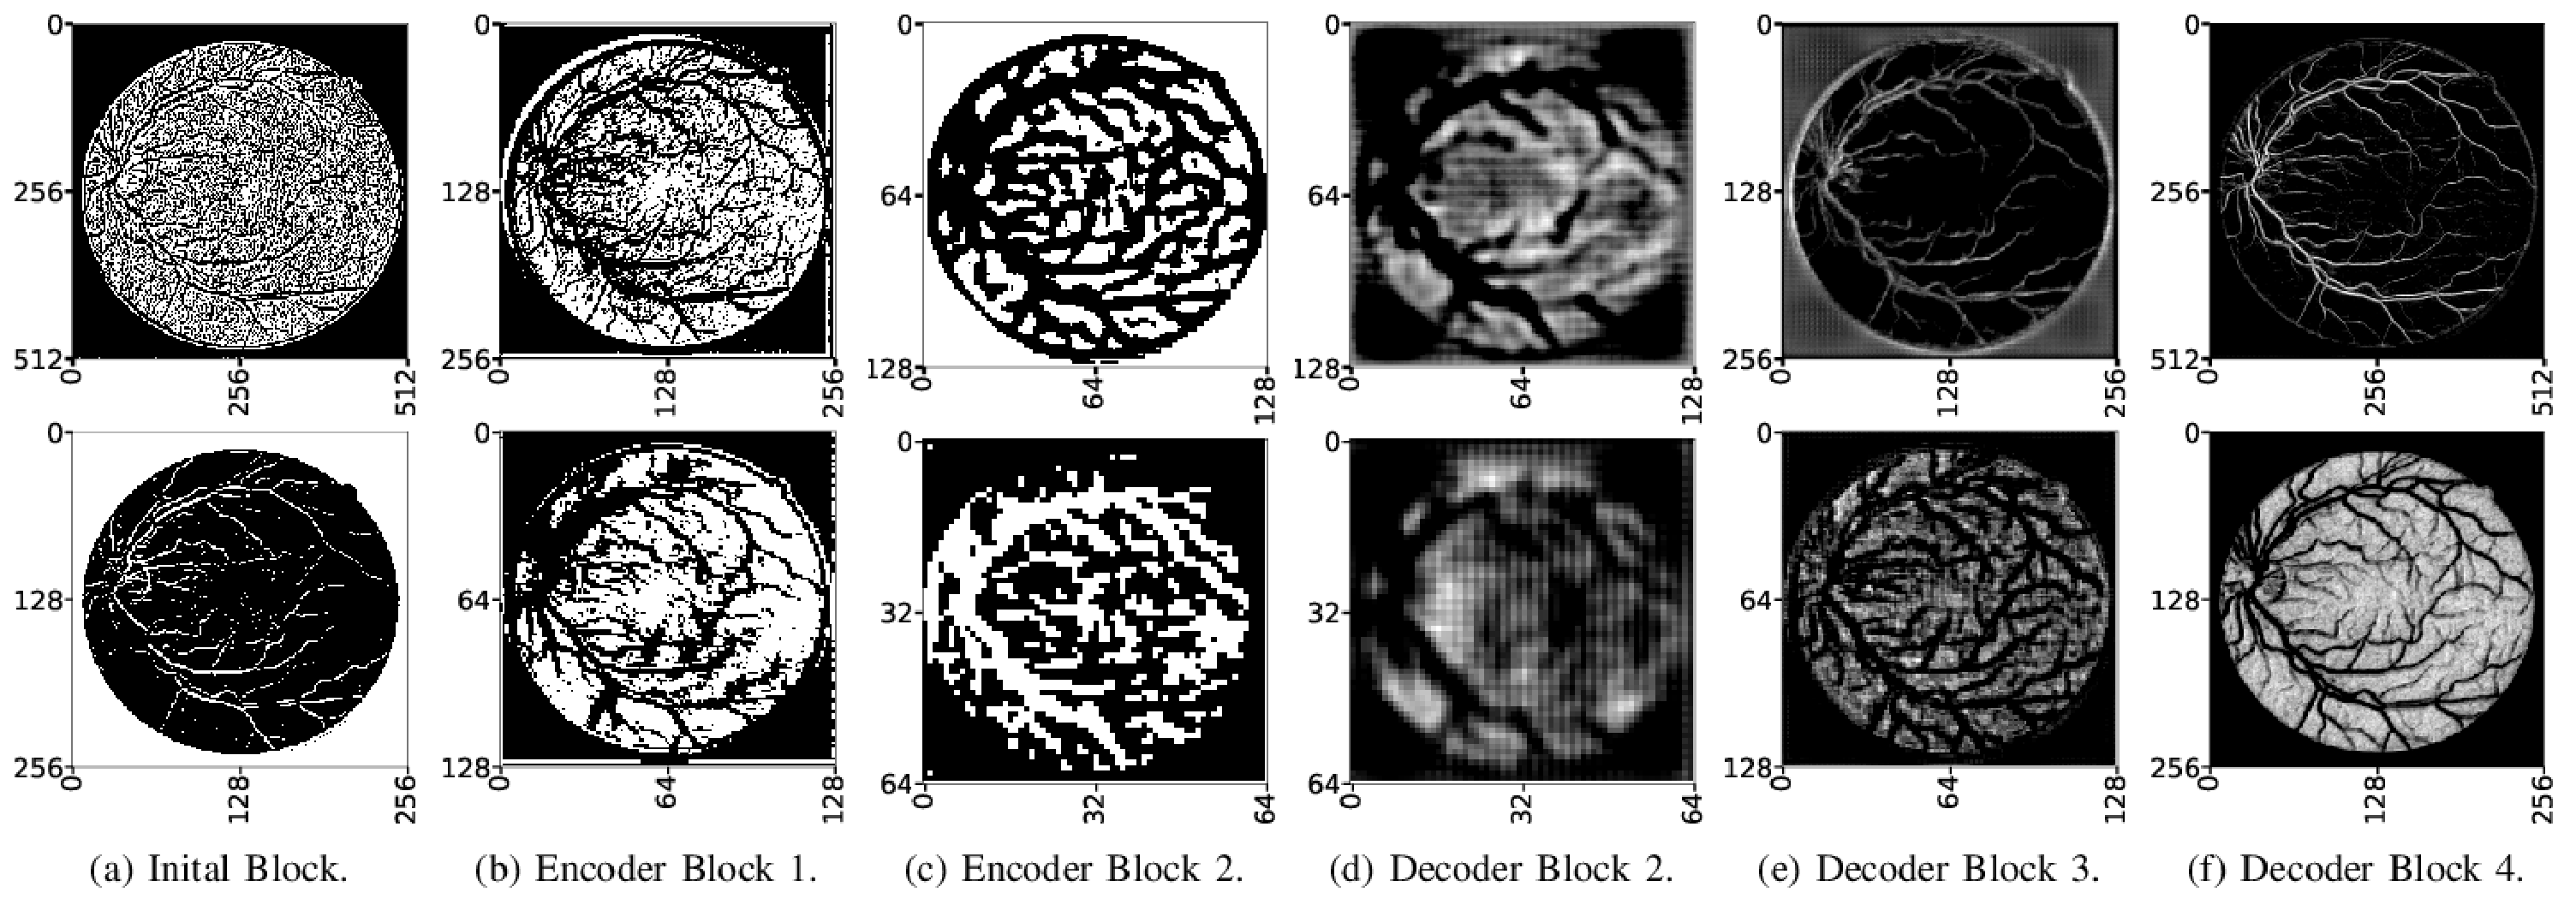
\includegraphics[width=180mm]{fig3.eps}
\caption{ }
\end{center}
\end{figure*}
\subsection{Implementation Details}
All the models are implemented using Keras.Models are trained for 10 epochs using Adam optimizer,with a learning rate of 1e-4 and batch size 8.Experiments have been conducted with Nvidia Geforce1080 Ti GPU - 11GB RAM.
\subsection{Evaluation Metrics}
\(1)\){\it Segmentation  evaluation: }Jaccard index and Dice similarity score are the most commonly used evaluation metrics for segmentation.
\begin{equation}
J a c c a r d(A, B)=\frac{|A \cap B|}{|A \cup B|},
\end{equation}

\begin{equation}
\operatorname{Dice}(A, B)=\frac{2|A \cap B|}{|A|+|B|},
\end{equation}
%\(2)\){\it Shape Similarity: }The shape similarity is measured by using the Hausdorff distance between the shape of segmented object and that of the ground truth object, defined as

%\begin{equation}
%H(A, B)=\max \left\{\sup _{x \in A} \inf _{y \in B}\|x-y\|, \sup _{y \in B} \inf _{x \in A}\|x-y\|\right\},
%\end{equation}
\(2)\){\it Intersection over Union(IoU): } Intersection over Union(IoU) is one of the standard measure performance measure for segmentation.Given a set of images, the IoU measure the similarity between the prediction and the ground truth per pixel.
\begin{equation}
IoU=\frac{TP}{TP+FN+FP},
\end{equation}
where TP, FP, FN denote the true positive,false positive and false negative numbers. This score is always between $0$ and $1$.
\subsection{Experimental Results}
In this section, we evaluate the segmentation performance of the performance of the proposed Octave Residual UNet . Preprocessingによる,ブラー画像の枚数は,表に示す.
\section{Conclusion}
\label{sec:con}
In this paper, we proposed a U-net like model with Octave Convolution layer 

\begin{figure*}[t]
\begin{center}
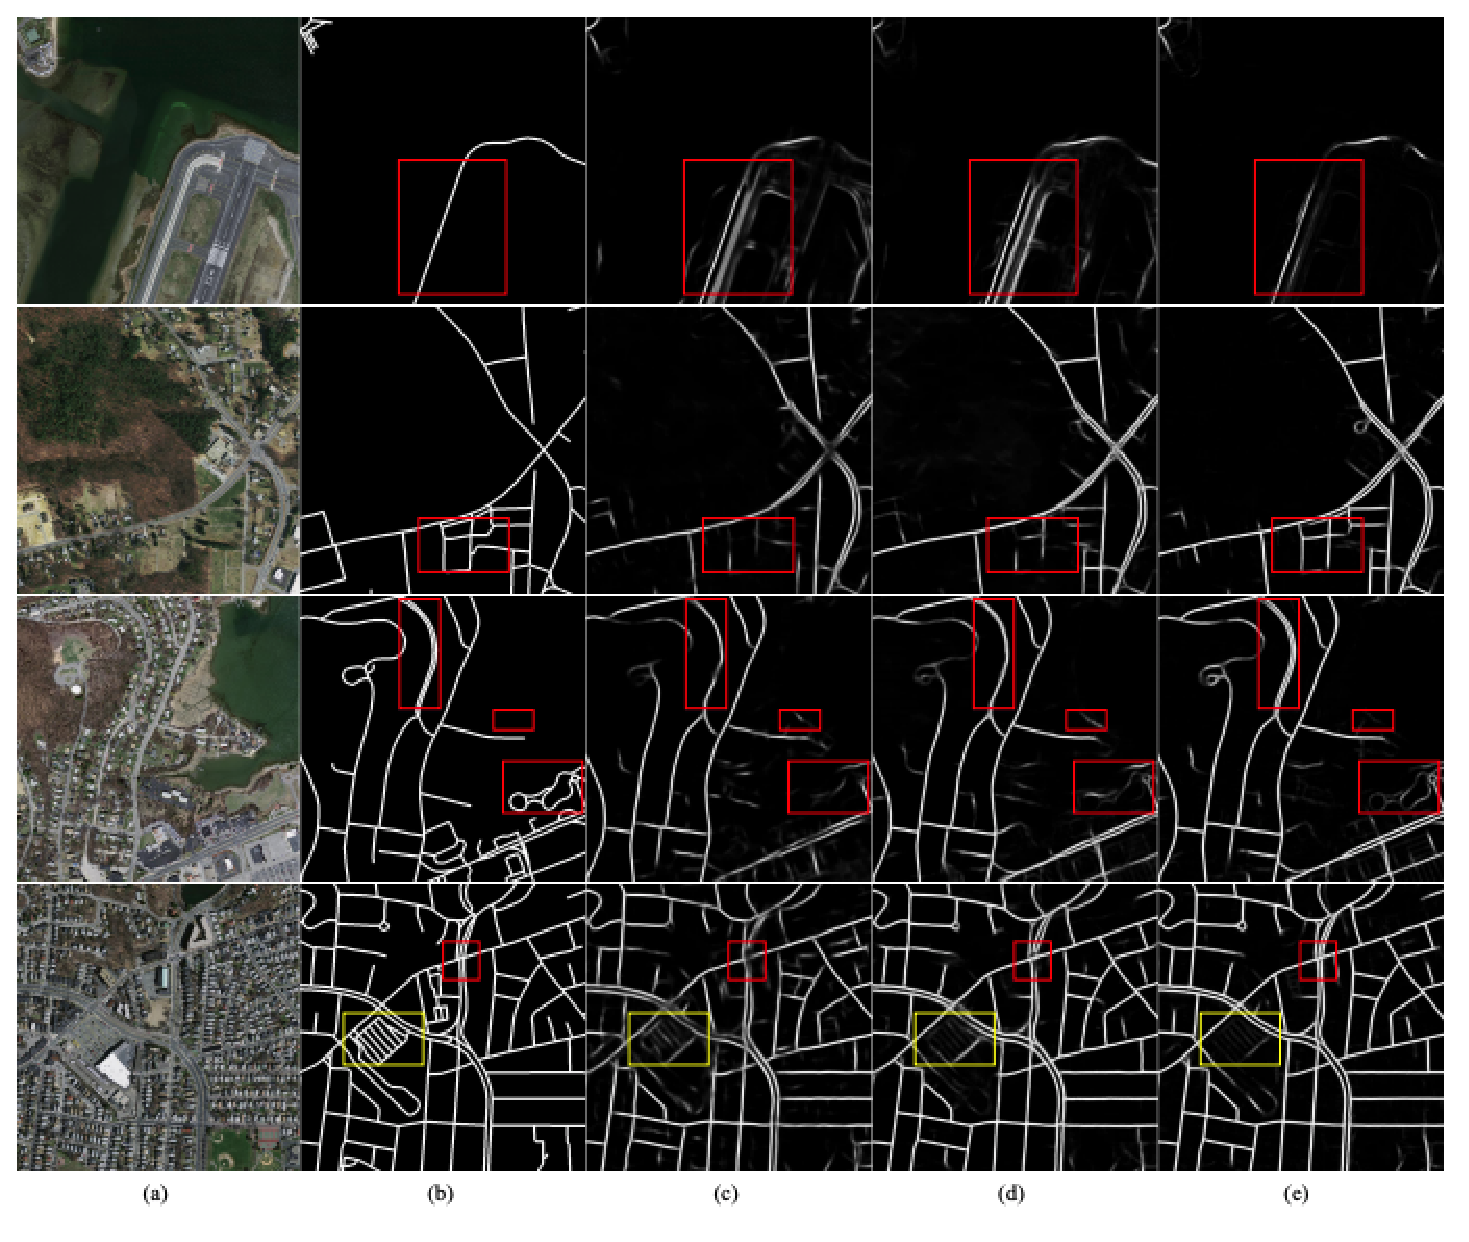
\includegraphics[width=180mm]{fig6.eps}
\caption{}
\end{center}
\end{figure*}
\vfill\pagebreak

\section{REFERENCES}
\label{sec:refs}


\end{document}
